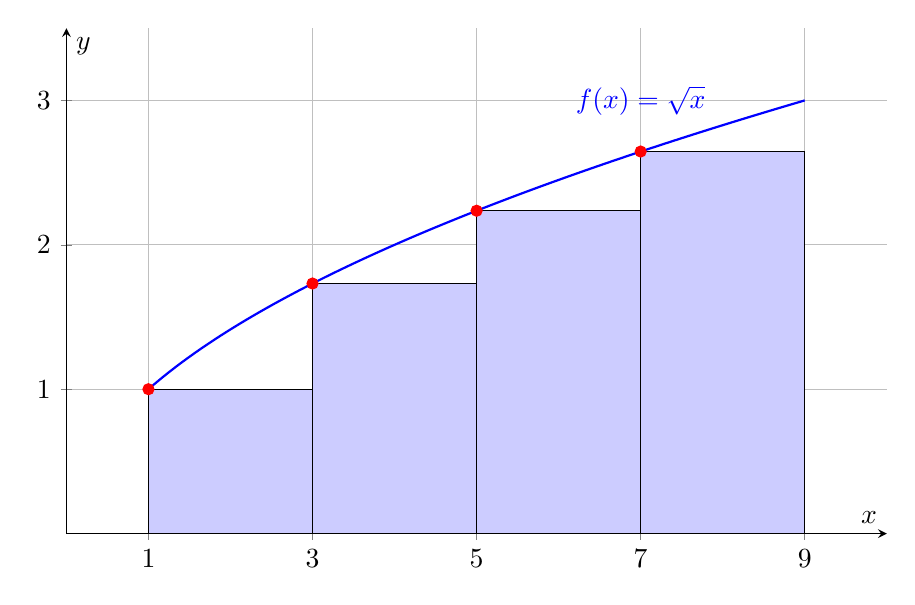
\begin{tikzpicture}
\begin{axis}[
    axis lines=center,
    xlabel=$x$, ylabel=$y$,
    domain=0:10, samples=100,
    xmin=0, xmax=10,
    ymin=0, ymax=3.5,
    width=12cm, height=8cm,
    xtick={1,3,5,7,9},
    ytick={1,2,3},
    grid=major
]
% Function plot
\addplot[blue, thick, domain=1:9] {sqrt(x)};
\node[blue] at (axis cs:7,3) {$f(x)=\sqrt{x}$};

% Left endpoint rectangles for n=4 on [1,9]
% Δx = 2
% Rectangles at x = 1, 3, 5, 7
\addplot[fill=blue!20, draw=black] coordinates {(1,0) (3,0) (3,1) (1,1) (1,0)};
\addplot[fill=blue!20, draw=black] coordinates {(3,0) (5,0) (5,1.732) (3,1.732) (3,0)};
\addplot[fill=blue!20, draw=black] coordinates {(5,0) (7,0) (7,2.236) (5,2.236) (5,0)};
\addplot[fill=blue!20, draw=black] coordinates {(7,0) (9,0) (9,2.646) (7,2.646) (7,0)};

% Mark the sample points
\addplot[only marks, mark=*, mark size=2pt, red] coordinates {(1,1) (3,1.732) (5,2.236) (7,2.646)};

\end{axis}
\end{tikzpicture}
